\title{Linear Algebra Fundamentals}
\date{}
\author{Michael Cowie}

\documentclass{article}

\usepackage{graphicx} % LaTeX package to import graphics
\graphicspath{{Math/linear_algebra/images/}} % Configuring the graphicx package

\usepackage[a4paper,margin=1.5cm,footskip=.5cm]{geometry}
\usepackage{amsmath}
\usepackage{parskip}

\usepackage{tocloft}
\renewcommand{\cftsecleader}{\cftdotfill{\cftdotsep}} % Adds dots to TOC

\setcounter{secnumdepth}{0} % sections are level 1

\begin{document}
\maketitle
\tableofcontents

\begin{center}
    \section{Fundamentals}
\end{center}

The fundamental, root-of-it-all building block for linear algebra is the vector, illustrated at figure \ref{fig1}.

\begin{figure}[h]
    \centering
    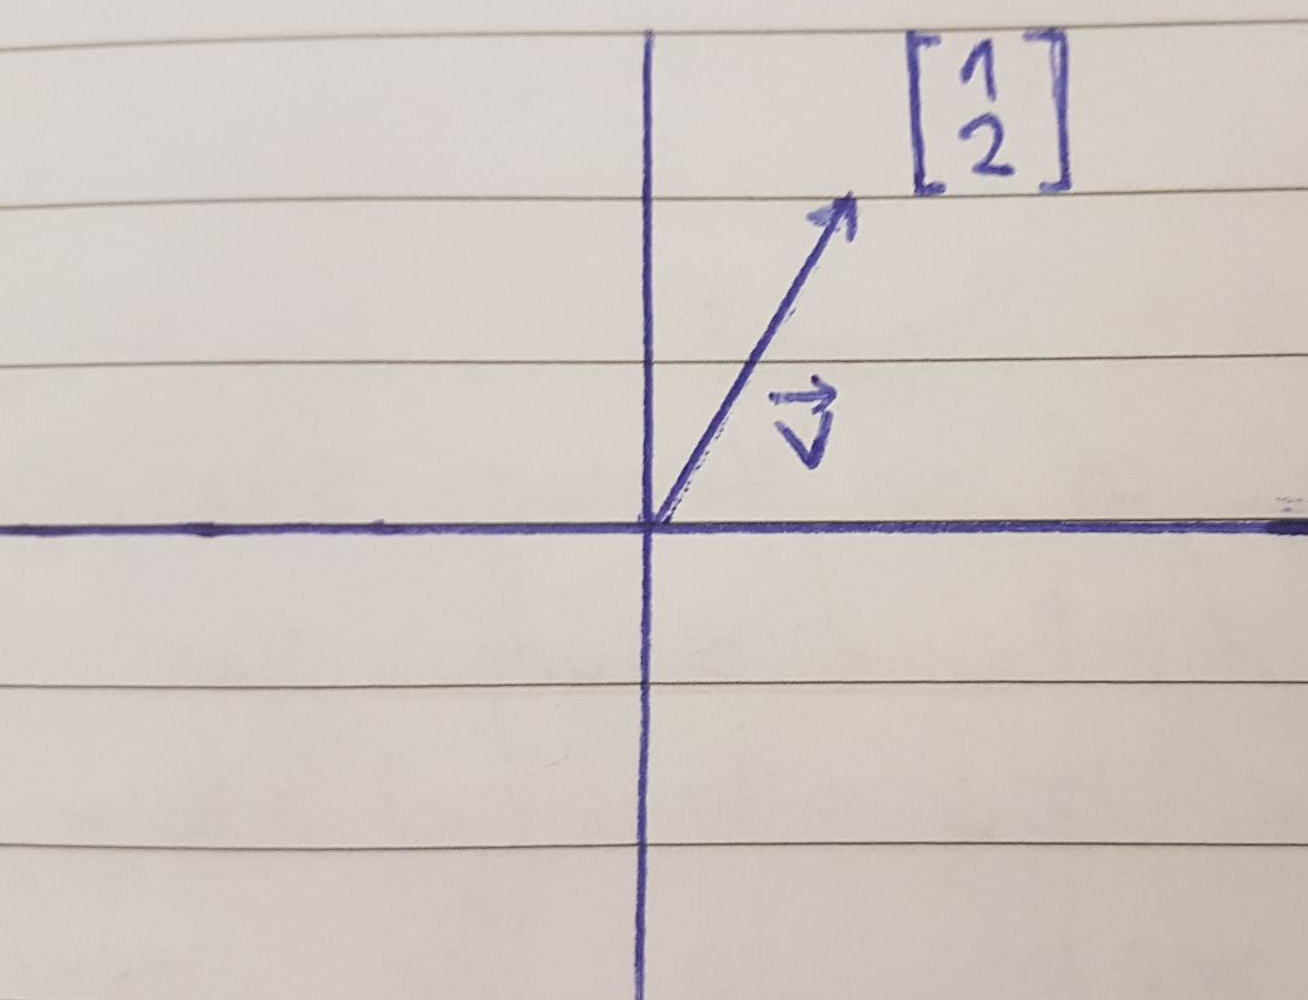
\includegraphics[width=0.5\textwidth, height=0.35\textwidth]{la_1.png}
    \caption{A basic vector}
    \label{fig1}
\end{figure}

What defines a given vector is its \textbf{length and the direction it is pointing in}, but as long as these two facts are the same, you can move it all around it is still \textbf{the same vector}. 

\begin{figure}[h]
    \centering
    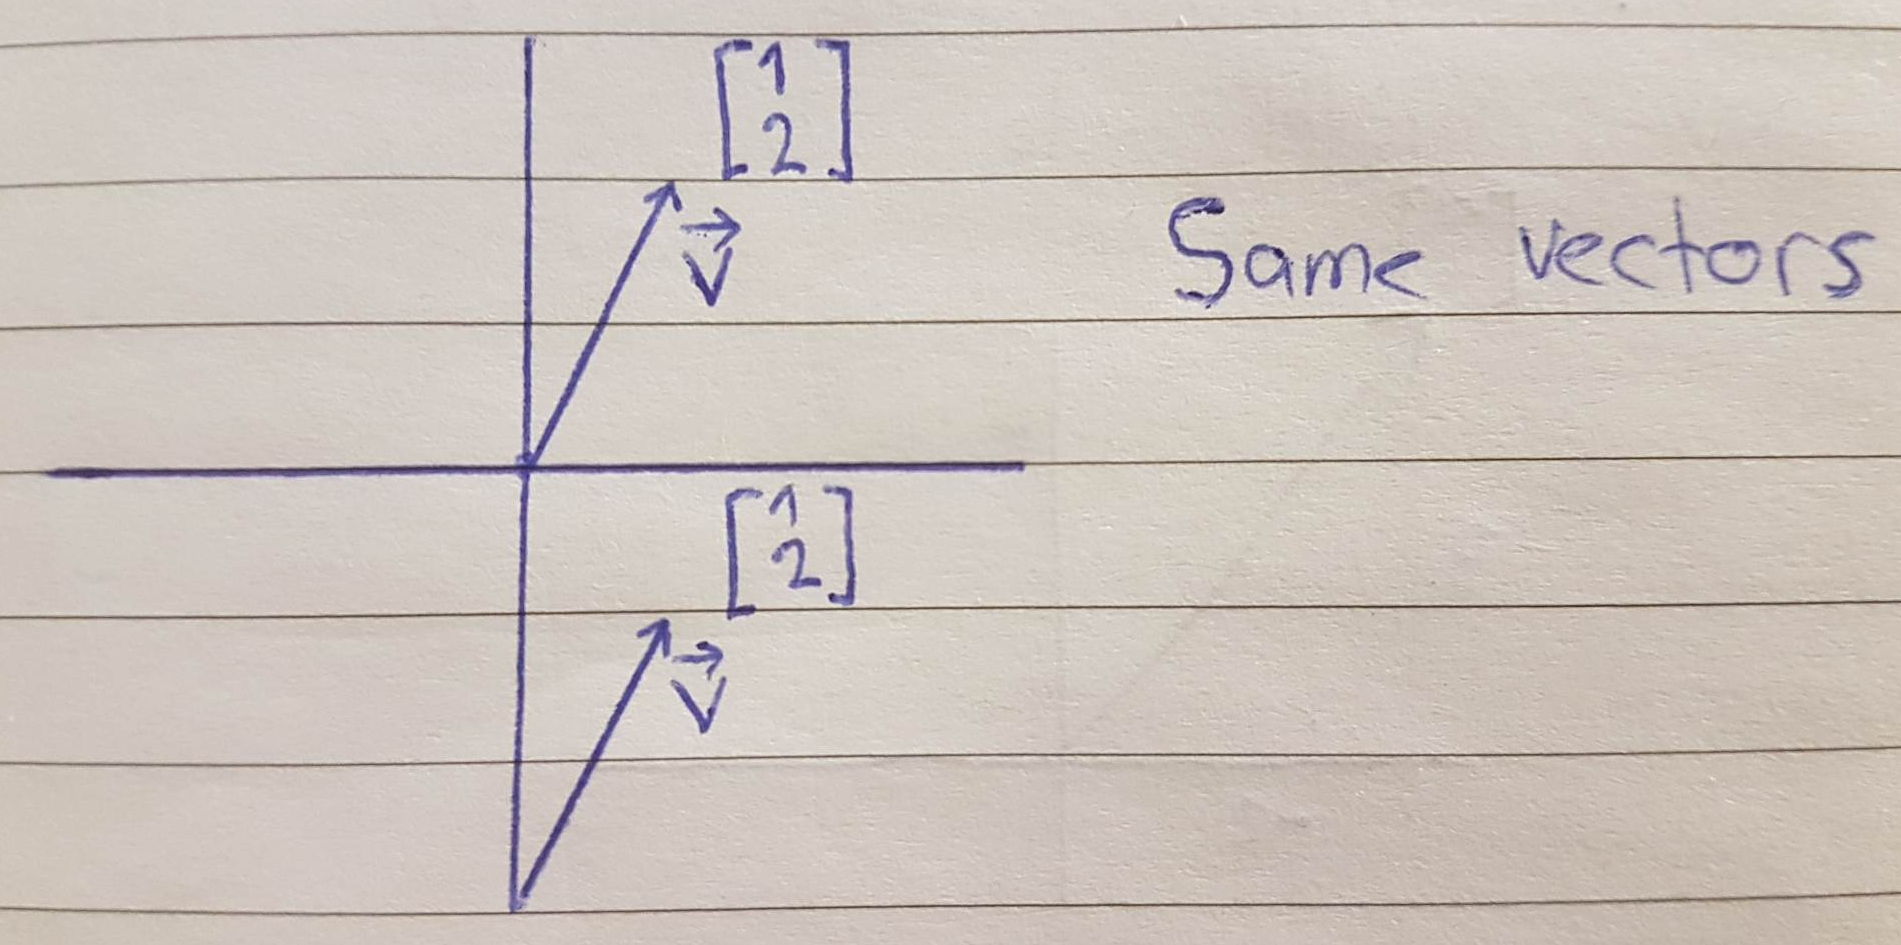
\includegraphics[width=0.5\textwidth, height=0.35\textwidth]{la_2.png}
    \caption{Identical vectors in different positions}
    \label{fig2}
\end{figure}

In linear algebra, it is \textbf{almost always the case that your vector will be rooted at the origin}. The coordinates of a vector are a pair of numbers that give instructions for how to get from the tail of the vector to the head (also called, the tip), represeted inside square brackets, e.g. $\begin{bmatrix} X \\ Y \end{bmatrix}$

The first number tells you now far to walk along the $X-axis$ and the second number tells you how far to walk parallel to the $Y-axis$.

To distinguish vectors from points, the convention is to write the pair of numbers vertically with square brackets around them.

\begin{itemize}
    \item $\begin{bmatrix} -2 \\ 3 \end{bmatrix}$ as a Vector
    \item $(-2, 3)$ as a Point
\end{itemize}

Every pair of numbers gives you \textbf{one and only one} vector.


\begin{figure}[ht!]
    \centering
    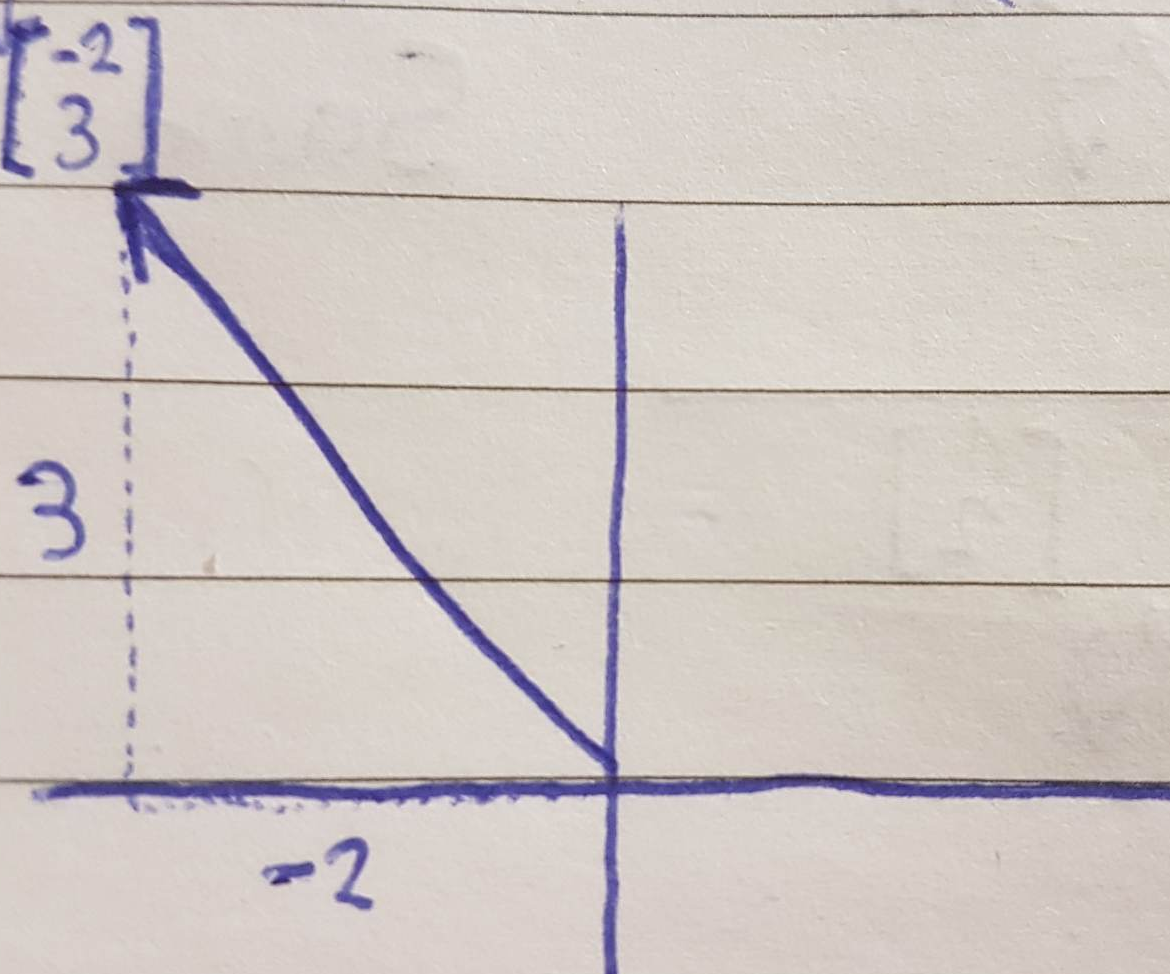
\includegraphics[width=0.5\textwidth, height=0.35\textwidth]{la_3.png}
    \caption{Example vector }
    \label{fig3}
\end{figure}

\begin{center}
    \section{Difference between Vector and a Point}    
\end{center}

The difference is precisely that between location and displacement.

\begin{itemize}
    \item Points are \textbf{locations} in space
    \item Vectors are \textbf{displacement} in space
\end{itemize}

An analogy with time works well.

\begin{enumerate}
    \item Times, (Also called instants or datetimes) are locations in time
    \item Durations are displacements in time
\end{enumerate}

So, in time;

\begin{itemize}
    \item 4:00pm, noon, midnight, 12:20am, etc... are all \textbf{times}
    \item +3 hours, -2.5 hours, +17 seconds, etc... are all \textbf{durations}
\end{itemize}

Notice how durations can be positive or negative; this gives them \textbf{direction} in addition to their pure scalar value. Now the best way to mentally distinguish times and durations is by the operations they support.

\begin{enumerate}
    \item Given a time, you can add a duration to get a new time, e.g. 3:00pm + 2 hours = 5:00pm
    \item You can subtract two times to get a duration, e.g. 7:00pm - 1:00pm = 6 hours
    \item You can add durations to get another, e.g. 3 hours + 50 minutes = 3 hours 50 minutes
\end{enumerate}

But, we cannot add two times, 3:15am + 4:00pm = ??

\newpage

\begin{center}
    \section{Space example for Vectors and Points}    
\end{center}

Let's carry the analogy over to now talk about space:

\begin{itemize}
    \item (3,5), (-2.25, 7), (0, -1), etc... are all \textbf{points}
    \item $\begin{bmatrix} 4 \\ -5 \end{bmatrix}$ is a \textbf{vector}, meaning 4 units east then 5 south, assuming north is up
\end{itemize}

Now we have exactly the same analogous operations operations in space as we did with time:

\begin{enumerate}
    \item You can add a point and a vector. Starting at (4, 5) and going $\begin{bmatrix} -1 \\ 3 \end{bmatrix}$ takes you to the point (3, 8)
    \item You can subtract two points to get a displacement between them: (10, 10) - (3, 1) = $\begin{bmatrix} 7 \\ 9 \end{bmatrix}$, which is the displacement you would take from the second location to get to the first.
    \item You can add two displacements to get a compound displacement: $\begin{bmatrix} 1 \\ 3 \end{bmatrix}$ + $\begin{bmatrix} -5 \\ 8 \end{bmatrix}$ = $\begin{bmatrix} -4 \\ 11 \end{bmatrix}$, that is going 1 step east then 3 north \textbf{and then} going 5 west then 8 north is the \textbf{same thing} as just going 4 west and then 11 north.
\end{enumerate}

But, you \textbf{cannot add two points}. In more concrete terms:

New Zealand + $\begin{bmatrix} 200km East \\ 7000km North \end{bmatrix}$ is another location (Point) somewhere on earth, but New Zealand + Australia makes no sense.


\begin{center}
    \section{Summary}    
\end{center}

To summarize, a location is where (or when) you are, and displacement is how to get from one location to another. Displacements have both magnitude (how far to go) and a direction (which in time, a one-dimensional space, is simply positive or negative). In space, locations are points and displacements are vectors. In time, locations are (points in) time, a.k.a instants and displacements displacements are durations.

\end{document}